\documentclass[border=5pt]{standalone}
\usepackage{tikz}
\usepackage{xcolor}

\definecolor{danger}{RGB}{220,53,69}
\definecolor{warning}{RGB}{255,193,7}
\definecolor{secondary}{RGB}{108,117,125}
\definecolor{success}{RGB}{40,167,69}
\definecolor{lightgreen}{RGB}{200,230,200}

\begin{document}
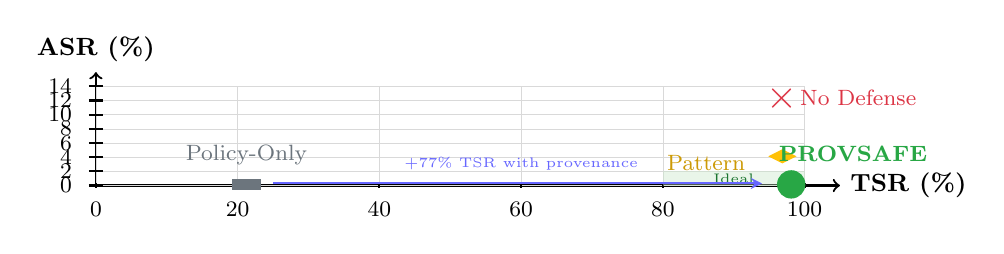
\begin{tikzpicture}[scale=0.09]
  % Axes
  \draw[thick, ->] (0,0) -- (105,0) node[right, font=\small\bfseries] {TSR (\%)};
  \draw[thick, ->] (0,0) -- (0,16) node[above, font=\small\bfseries] {ASR (\%)};
  
  % Grid
  \draw[gray!30, very thin] (0,0) grid[xstep=20, ystep=2] (100,14);
  
  % Axis labels
  \foreach \x in {0,20,40,60,80,100} {
    \draw[thick] (\x,-0.3) -- (\x,0.3);
    \node[below, font=\footnotesize] at (\x,-1) {\x};
  }
  \foreach \y in {0,2,4,6,8,10,12,14} {
    \draw[thick] (-1,\y) -- (1,\y);
    \node[left, font=\footnotesize] at (-2,\y) {\y};
  }
  
  % Ideal region (high TSR, low ASR)
  \fill[lightgreen, opacity=0.4] (80,0) rectangle (100,2);
  \node[font=\tiny, success!70!black] at (90,1) {Ideal};
  
  % Data points
  % No Defense: TSR=96.88%, ASR=12.34%
  \node[danger, font=\Large] at (96.88, 12.34) {$\times$};
  \node[right, font=\footnotesize, danger] at (98, 12.34) {No Defense};
  
  % Pattern Filter: TSR=96.88%, ASR=3.12%
  \fill[warning] (96.88, 3.12) -- (94.88, 4.12) -- (96.88, 5.12) -- (98.88, 4.12) -- cycle;
  \node[left, font=\footnotesize, warning!80!black] at (93, 3.12) {Pattern};
  
  % Policy-Only: TSR=21.25%, ASR=0%
  \fill[secondary] (21.25-2, 0.1-0.8) rectangle (21.25+2, 0.1+0.8);
  \node[above, font=\footnotesize, secondary] at (21.25, 1.5) {Policy-Only};
  
  % PROVSAFE: TSR=98.12%, ASR=0.16%
  \fill[success] (98.12, 0.16) circle (2);
  \node[above right, font=\footnotesize\bfseries, success] at (95, 2) {\textbf{PROVSAFE}};
  
  % Arrow showing improvement from Policy-Only to PROVSAFE
  \draw[thick, ->, >=stealth, blue!60] (25, 0.3) -- (94, 0.3);
  \node[font=\tiny, blue!60, above] at (60, 0.8) {+77\% TSR with provenance};
  
\end{tikzpicture}
\end{document}
